%!TEX root =  main.tex
\section{Performance evaluation}
\label{sec:experiments}

In this section, we evaluate \dynastar{} according to various metrics,
under a variety of different operational parameters.
We ran a number of experiments using two benchmarks: the TPC-C benchmark and
\appname{} social networking service described in the previous section.
Our experiments show that \dynastar{} is able to rapidly adapt to changing 
workloads, while achieving throughputs and latencies far better than the existing
state-of-the-art approaches to state machine replication partitioning.


\subsection{Experimental environment}
\label{sec:evaluation:setup}

We conducted all experiments on a cluster with two types of nodes: (a)
HP SE1102 nodes, equipped with two Intel Xeon L5420 processors running
at 2.5 GHz and with 8 GB of main memory, and (b) Dell SC1435 nodes,
equipped with two AMD Opteron 2212 processors running at 2.0 GHz and
with 4 GB of main memory. The HP nodes were connected to an HP
ProCurve 2920-48G gigabit network switch, and the Dell nodes were
connected to another, identical switch. Those switches were
interconnected by a 20 Gbps link.  All nodes ran CentOS Linux 7.1 with
kernel 3.10 and had the OpenJDK Runtime Environment~8 with the
\mbox{64-Bit} Server VM (build 25.45-b02). In all experiments, the oracle 
had the same resources as every other partition: 2 replicas and 3 acceptors 
(in total five nodes per partition).


\subsection{Methodology and goals}
\label{sec:evaluation:methodology}

%In order to show the scalability of our approach we tested the performance as the 
%number of partitions increases, and performance as the size and complexity of the graph grows.
The experiments seek to answer the following questions:
\begin{itemize}
\item \emph{What is the impact of repartitioning on a static workload and on a dynamic workload?}
\item \emph{How does partitioning affect performance when the workload grows with the number of partitions and when the workload has constant size?}
\item \emph{How does \dynastar performance compare to other approaches?} 
\item \emph{How does \dynastar perform under dynamic workloads?}
\item \emph{What is the performance of the oracle?}
\end{itemize}

\paragraph*{Performance metrics.}
%
The latency was measured as the end-to-end time between issuing the
command, and receiving the response.  Throughput was measured as the
number of posts/second or transactions/second that the clients were able to send.

\subsection{TPC-C benchmark}
\label{sec:evaluation:tpc-c}

In the experiments in this section, we deploy as many partitions as the number of warehouses.

\begin{figure}[ht!]
  \centering
    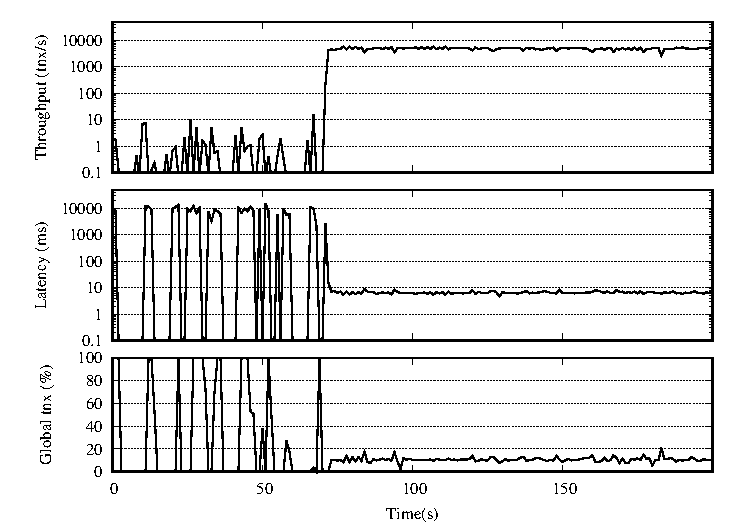
\includegraphics[width=\columnwidth]{figures/experiments/tpcc-repartitioning/tpcc-repartitioning}
  \caption{Repartitioning on \dynastar}
  \label{fig:tpcc_repartitioning}
\end{figure}

\paragraph{The impact of graph repartitioning.}
In order to assess the impact of state partitioning on performance, we ran the TPC-C benchmark on an un-partitioned database.  Figure ~\ref{fig:tpcc_repartitioning} 
shows the performance of \dynastar with 8 warehouses and 8 partitions.
At the first part of the experiment, all the variables are randomly distributed across all partitions.
As a result, almost every transaction accesses all partitions. Thus every transaction 
required coordination between partitions, and objects were constantly moving back and forth. 
%In addition, transactions from different clients were blocked by the others, 
%made the time it took for executing one transaction remarkably high.
This can be observed in the first 45 seconds of the experiment depicted in Figure ~\ref{fig:tpcc_repartitioning}: low throughput (i.e., a few transactions executed per second), high latency (i.e., several seconds), and a high percentage of cross-partition transactions.

%In addition to that, when a partition takes part in an execution of a transaction, 
%if another command access variables that are being accesses by the ongoing command will 
% be blocked until the previous command finish

After 45 seconds, the oracle computed a new partitioning based on previously executed transactions and instructed the partitions to apply the new partitioning.
When the partitions delivered the partitioning request, they exchanged objects to achieve the new partitioning.
% During this process, servers didn't execute any other transactions, thus the throughput decreased 
% to 0, and the average latency was not applicable. 
It takes about 10 seconds for partitions to reach the new partitioning.
However, during the repartitioning servers continue to execute transactions.
After the state is relocated, most objects involved in a transaction
can be found in a local partition, which considerably increases performance and reduces latency. 

\begin{figure}[ht!]
  \centering
    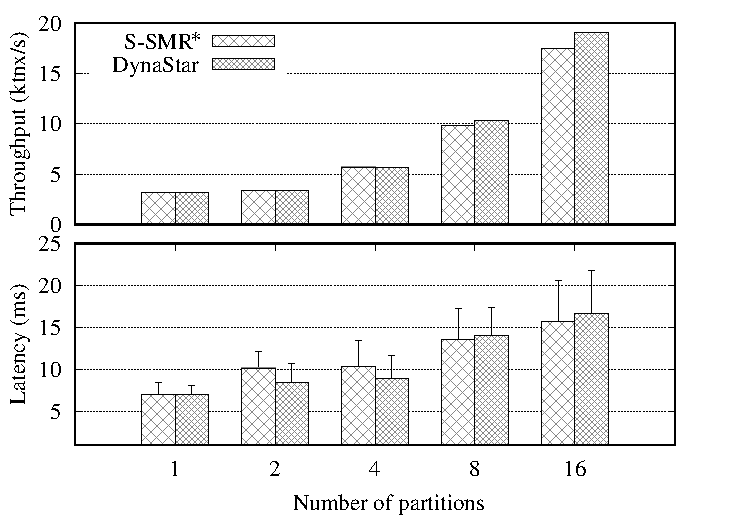
\includegraphics[width=\columnwidth]{figures/experiments/tpcc-scaling-tp-lat/tpcc-scaling-tp-lat}
  \caption{Performance scalability with TPC-C.}
  \label{fig:tpcc_scaling}
\end{figure}
\paragraph*{Scalability.}
In order to show how \dynastar scales out, we ran experiments with 1, 2, 4, 8 and 16 partitions. 
%We also added warehouses while adding partitions to demonstrate using 
%\dynastar to grow an application by adding more hardware. 
We used sufficient clients to  saturate the throughput of the system in each experiment. 
Figure ~\ref{fig:tpcc_scaling} shows the peak throughput of \dynastar as we vary the 
number of partitions. 
Notice that we increase the state size as we add partitions (i.e., there is one warehouse per partition).
The result shows that \dynastar is capable of applying
a partitioning scheme that leads scalable performance.


\subsection{Social network}

%\paragraph*{Workloads.}
We used the Holme-Kim model~\cite{holme-kim} to generate the social 
graphs used in the experiments. We created power-law graphs (also
known as scale-free graphs) with a clustering coefficient varying from
0.6 to 1, which represent the geometric structures of social
networks. The coefficient is the probability that whenever an edge
$(v, w)$ is added to the graph, $v$ connects to some neighbour of $w$.
In the experiments, we tested graphs with 100000 users. We characterize
different workloads by varying the percentage of edge-cuts.  For
example, a graph with a 5\% edge cut means that 5\% of the total edges
in the graph have connected vertices located in different partitions.
%Graphs with 0\% of edge-cuts have \emph{strong locality}.


% \paragraph*{Command generation.}
% %
% As a workload for the social graph, we have simulated clients,
% and each client issues a sequence of post
% commands.  For each command, the client selects a random node as
% the poster.  We focused on post commands, since they may access
% multiple partitions. Each client operates synchronously,
% waiting for a response from the storage (i.e., in a closed loop).

\begin{figure*}[ht!]
	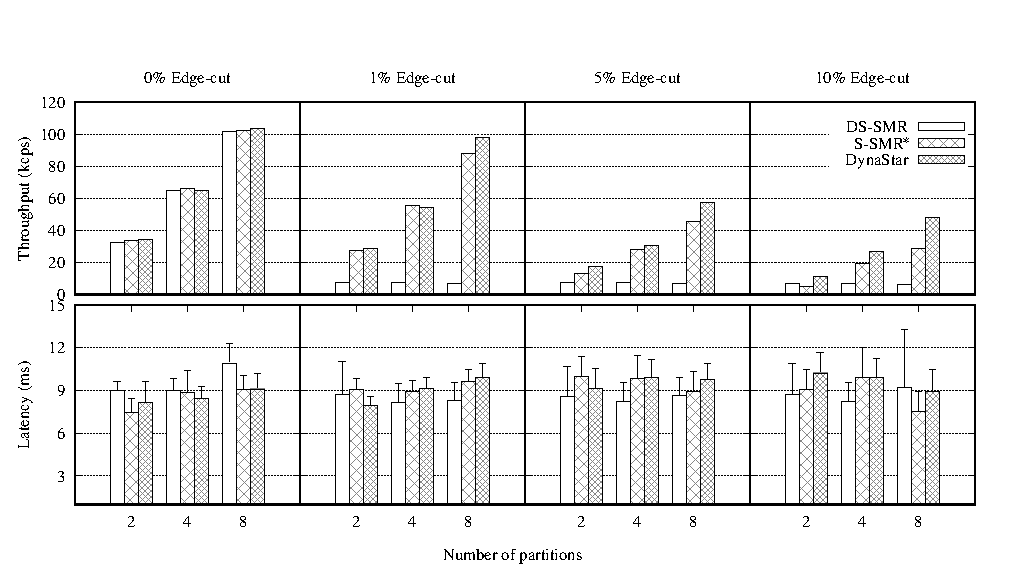
\includegraphics{figures/experiments/social-network-tp-lat/social-network-tp-lat}
	\caption{Throughput and latency for different partition numbers. 
  Throughput is in thousands of commands per second (kcps). 
  Latency for $\approx$75\% peak throughput is in milliseconds (bars show average, whiskers show 95-th percentile).}
	\label{fig:varying_edge_cut}
\end{figure*}




% \paragraph*{Operational parameters.}
% %
% With post commands, the frequency of single-partition
% vs. multi-partition commands depends on the number of partitions, the
% geometry of the social graph, and the technique used to partition the
% data. We ran experiments with 2 to 8 partitions.  To vary the
% geometry, we generated graphs with varying percentages of edge-cuts as
% computed by METIS on a static graph. Our experiments used graphs with
% 0\%, 1\%, 5\% and 10\% of edge cuts. We configured METIS to keep the size of 
% the most unbalanced partition up to 30\% more than the average partition size.
% %As already mentioned, we compared three strategies: \ssmr{}, \dssmr, and \dynastar.


\paragraph*{\dynastar vs. alternative techniques.}
\label{sec:evaluation:results}

Figure~\ref{fig:varying_edge_cut} shows the peak throughput and latency for $\approx$75\% of peak throughput (average and 95-th percentile) of the three techniques, 
as we vary the number of partitions for social networks with different percentages of edge cuts.

All three techniques perform similarly when there are no cross-partition commands after
the graph is perfectly partitioned. This happens because no more moves occur in
\dynastar or \dssmr, and no synchronization among partitions is
necessary for \ssmr in this case. 
Consequently, all three schemes scale remarkably well, and
the difference in throughput between each technique is due to the implementation of each one.
%Although \dynastar and DS-SMR have comparable performance, they differ in an important way. 
%As shown in Figure~\ref{fig:motivation} (top left graph) for 4 partitions, \dynastar converges 
%to maximum throughput after 20 seconds from the beginning of the execution, while it takes 
%DS-SMR (decentralized dynamic scheme) about 80 seconds to converge.
%This means that \dynastar can react to workload changes more rapidly than DS-SMR.

With social networks with edge cut percentage greater than zero \dssmr\ performance decreases significantly.  
This happens because in such cases, objects in \dssmr\ are constantly being moved back and forth between partitions 
without converging to a stable configuration.
%(see also Figure~\ref{fig:motivation}, graph on the bottom right, for 4 partitions). 
In contrast, for \dynastar and \ssmr with an optimized partitioning, we see that the throughput scales with the number of partitions in experiments with up to 10\% of edge cuts. 
%With 10\% of edge cuts and above, the overhead from moves (in \dynastar) and cross-partition commands (in S-SMR) outweighs the gains from additional partitions.



\paragraph*{The ideal number of partitions.}
\label{sec:evaluation:results}

While in the previous section we considered executions with a fixed percentage of edge cuts.
%, as we increased the number of partitions 
%(by adjusting the social graph clustering coefficient),
We now consider a fixed social network graph and vary the number of partitions.
Increasing the number of partitions with a fixed graph introduces a tradeoff.
On the one hand, additional partitions improve performance as there are more resources to execute posts.
On the other hand, the number of edge cuts increases with the number of partitions, which hurts performance as there are additional operations involving multiple partitions.
We evaluate the performance of \dynastar, \dssmr\ and \ssmr with an optimized partitioning.% when subject to this tradeoff. 

\begin{figure}[ht]
	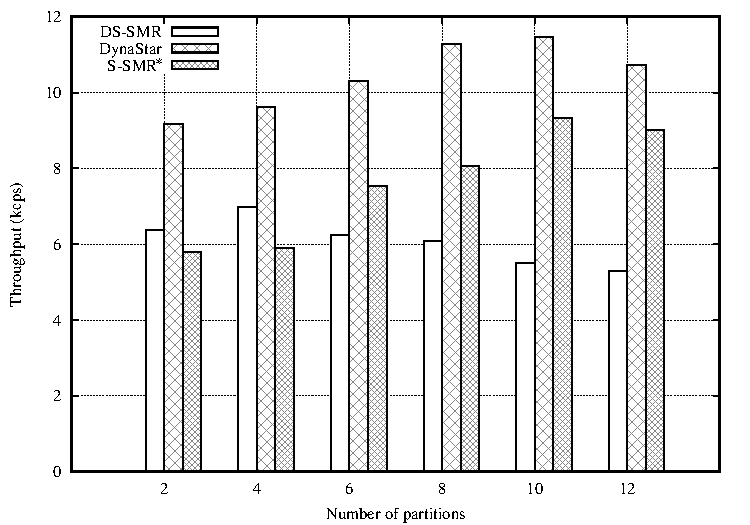
\includegraphics[width=0.95\columnwidth]{figures/experiments/social-network-ideal-partition/social-network-ideal-partition}
	\caption{Performance scalability with social network.}
	\label{fig:4p1p_varying_partition_size}
\end{figure}

Figure~\ref{fig:4p1p_varying_partition_size} shows that \dynastar and optimized \ssmr throughput scale up to ten partitions, after which performance decreases. \dssmr\ throughput decreases gradually as we increase partitions, since the chance that objects are spread between partitions also increases.
% For each configuration, we computed the percentage of edge cuts and found that for 2, 3, 4, 6 and 8 partitions the percentages were respectively 
% 0.13\%, 0.88, 1.06\%, 2.28\% and 2.67\%.
Notice that only post operations are subject to this tradeoff since they may involve multiple partitions.
The most common operation in social networks is the request to read a user timeline. This is a single-partition
command in our application and as a consequence it scales linearly with the number of partitions.


\begin{figure*}[h!]
  \centering
  \begin{subfigure}[b]{0.45\textwidth}
    \centering
    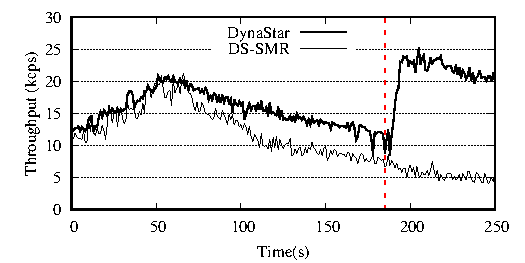
\includegraphics[width=0.95\columnwidth]{figures/experiments/social-network-dynamic/social-network-dynamic}
    \caption{\dynastar versus DS-SMR}
  \end{subfigure}
  \begin{subfigure}[b]{0.45\textwidth}
    \centering
    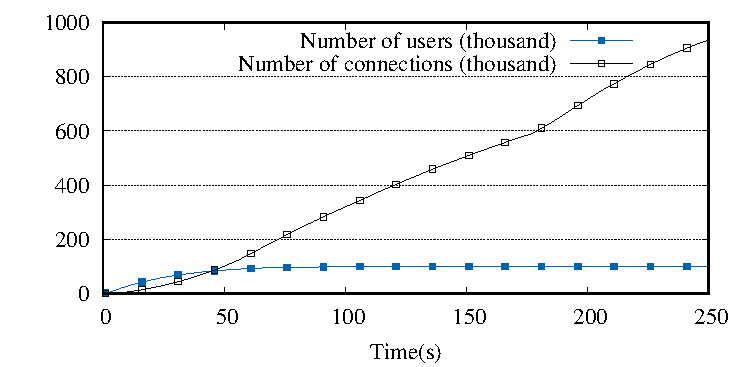
\includegraphics[width=0.95\columnwidth]{figures/experiments/social-network-dynamic/social-network-dynamic-structure}
    \caption{The creation of a social network graph}
  \end{subfigure}
    \caption{Performance under dynamic workload (four partitions and 10\% of edge cuts).}
	\label{fig:dynamic_load_tput}
\end{figure*}

% We can draw similar results about the latency of the three strategies (Figure~\ref{fig:varying_edge_cut}, graphs on the bottom).
% The large number of move operations in DS-SMR with social graphs that cannot be perfectly partitioned result in increased latency.

\paragraph*{Performance under dynamic workloads.}

Figure~\ref{fig:dynamic_load_tput} (left) depicts performance of an evolving social network.  
We started the system with an empty graph. Then clients
continuously create users and connections between them during the experiment
by executing the follow command.
The rate at which users and connections are created is shown in Figure~\ref{fig:dynamic_load_tput} (right).
The oracle monitors changes in the
graph's structure and was configured to trigger a repartitioning after receiving a number of hints
%(object creating and connecting)
from the partitions.
%after all users were in the system and after 300 seconds into the execution.
%when the number of changes exceed a threshold.  
%When the repartitioning took place, the partitioning became better and helped the throughput increase.
%We also show the behavior of DS-SMR.
When the repartitioning takes place, around 122 seconds into the execution, the previously random user mapping got a better location from the oracle.
After the repartitioning, the objects are moved to a better partition.
The partitioning became better and thus the throughput increased.
We also show the behavior of DS-SMR.
When few connections are in the system, most of the posts are single-partition commands, but as connections are added, moves are needed to execute posts and performance decreases quickly.

%\begin{figure}[ht]
%	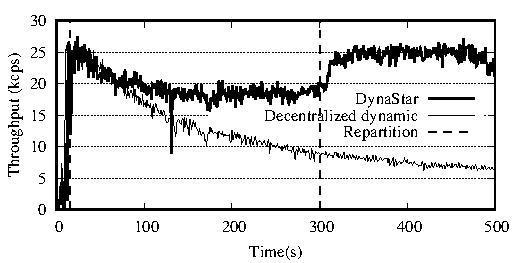
\includegraphics{figures/experiments/dynamicload-tp-move-4p}
%	\caption{Adding nodes and repartitioning dynamically}
%	\label{fig:dynamic_load_tput}
%\end{figure}
%\begin{figure}[ht]
%	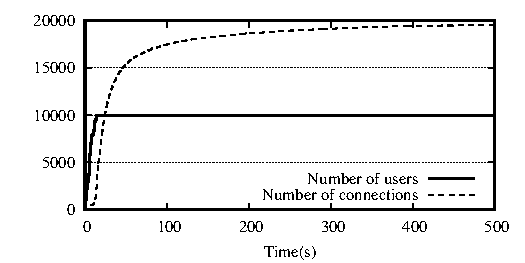
\includegraphics{figures/experiments/dynamicload-graph-structure}
%	\caption{Changes in dynamic workloads}
%	\label{fig:dynamic_load_changes}
%\end{figure}

\subsection{The performance of the oracle}

\dynastar differs from \dssmr\ in the sense that it uses an oracle
that maintains a global view of the workload graph. The oracle allows
\dynastar to make better choices about data movement, resulting in an overally
better throughput and lower latency. However, introducing a centralized
component in a distributed system is always a cause for some skepticism,
in case the component becomes a bottleneck, or a single point of failure. 
To cope with failures, the oracle is implemented as a replicated partition. 
We conducted two experiments to evaluate if the \dynastar oracle is a bottleneck to
system performance. The results show that the load on the oracle is
low, suggesting that \dynastar scales well.


The first experiment assesses the scalability of the METIS algorithm only.
We measured the time to compute the partitioning solution, and
the memory usage of the algorithms for increasingly large graphs. 
The results, depicted in Figure~\ref{fig:metis_size_time}, show that METIS scales
linearly in both memory and computation time on graphs of up to 10 million vertices.

\begin{figure}[ht!]
  \centering
    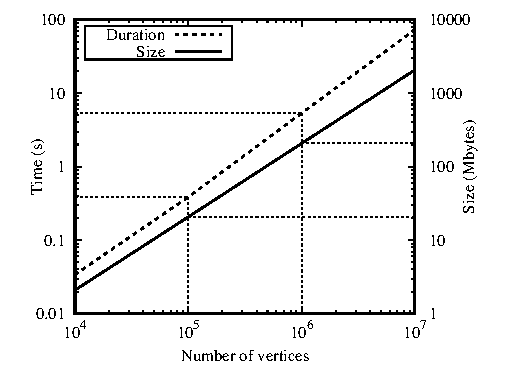
\includegraphics[width=\columnwidth]{figures/metis_size_time}
	\caption{METIS processor and memory usage.}
	\label{fig:metis_size_time}
\end{figure}

The second experiment evaluates the oracle in terms of CPU load over
time, for varying numbers of partitions. The results are shown in
Figure~\ref{fig:cpu_oracle}. The load is higher in the
beginning of the experiment, when the clients had not yet cached the
requests and the oracle was busy moving the states. However, the load diminishes rapidly, and remains relatively
low over time. This is because access to the oracle is necessary only
when clients have an invalid cache or when a repartition happens. These experiments
suggest that the oracle would not become a bottleneck.% for reasonably large
%deployments.

\begin{figure}[ht]
	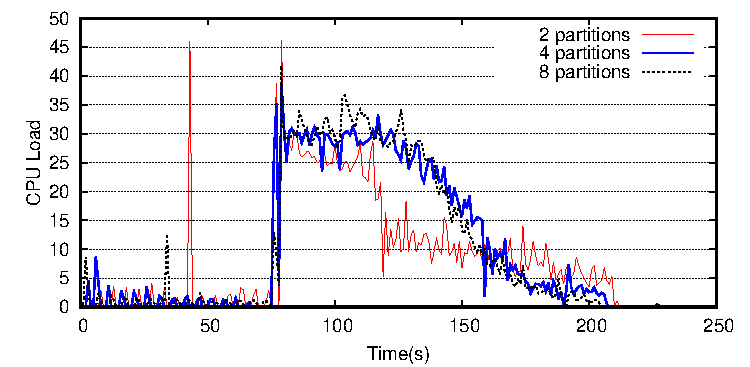
\includegraphics[width=\columnwidth]{figures/experiments/social-network-oracle-load/social-network-oracle-load}
  \caption{CPU load in the oracle (5\% of edge cuts).}
	\label{fig:cpu_oracle}
\end{figure}

